%!TEX root = ../dissertation.tex
\begin{savequote}[75mm]
Science may be described as the art of systematic over-simplification.
\qauthor{Karl Popper}
\end{savequote}

\chapter{Previous Work}
\label{chap:previous_work}
\newthought{Several works have addressed tasks that involve CV and NLP}, such as object detection based on natural language expressions \cite{hu_natural_2015}\cite{guadarrama_understanding_2016}, image captioning \cite{hendricks_deep_2015}\cite{gan_semantic_2016}\cite{johnson_densecap:_2016}\cite{yang_review_2016} and visual question answering (VQA) \cite{goyal_making_2016}\cite{zhu_visual7w:_2015}\cite{krishna_visual_2016}\cite{agrawal_vqa:_2015}\cite{teney_graph-structured_2016}. Nevertheless, the standard way of processing both types of information jointly has never been clearly established, since visual and linguistic data have properties that make them fundamentally different, \textit{i.e.} the former has spatial meaning and no sequentiality while the latter does not contemplate space but has a sequential nature. Hence, each work in this sub-field has proposed a particular way of addressing each task.

On this chapter, we intend to describe three model architectures that mix both language referring expressions and vision inputs to produce a segmentation mask. While two of them \cite{hu2016segmentation} \cite{liu2017segmentation} try to solve the task by merging language and vision representations by defining a new, synthetic entity that describes the relation between both, the third one \cite{li2017cvpr} tr aims to map one domain to the other \textit{i.e.,} map language features to the visual filter space to accomplish object tracking on videos based on referring expressions.

\section{Segmentation from Natural Language Expressions}
On this work \cite{hu2016segmentation}, the authors process visual and natural language information through separate neural networks: a CNN extracts visual features from the image while an LSTM is applied to the natural language query. Strided convolutions and pooling operations in the CNN progressively downsample the feature maps to a low resolution output while producing a large receptive field size for neurons in the final layers.

Thus, the authors use a modified pre-trained VGG-16 \cite{DBLP:journals/corr/SimonyanZ14a} as a feature extractor whose last three fully-connected layers were replaced by three convolutional layers. Given an image of height \textit{H} and width \textit{W},  the output of such a fully convolutional network (FCN) is a spatial feature map of dimensions $h$ and $w$  with $D$ channels at each spatial location. The strided convolutions and pooling operations, while reducing the size of the image  to $h = \frac{H}{32}$ and $w = \frac{W}{32}$, also provide the units of the final response map with a large receptive field. At each spatial location, $\ell^2$-normalization is applied in search for a \textit{more robust feature representation}. 

Additionally, to explicitly model localization in the network (\textit{i.e.} help the network reason about queries containing localization information), relative coordinates are concatenated at each spatial location in the feature map obtained by the CNN, thus obtaining a final visual feature map, with $D + 8$ channels. 

On the other hand, language information is processed by tokenizing each word with a Word Embedding (WE) and passing each of these through a Long Short-Term Memory (LSTM) cell until the end of the sentence is reached. The last hidden state of the LSTM, which is expected to hold an overall representation of the expression's concept, is $\ell^2$-normalized and concatenated along the channel axis at \textit{each spatial location} of the feature representation that was obtained from the FCN module. If the hidden state of the LSTM is of length $L$, the concatenation of the linguistic and visual representation is of shape $(L + D + 8) \times h \times w$. Merging of visual and natural language information is done by concatenating the output of the LSTM to the visual feature map at each spatial location.

Finally, two $1\times1$ convolution layers with ReLU nonlinearities in between are applied for final classification. The ground truth mask is downsampled to have the same dimensions as the output, so that they can be directly compared. The loss function is defined as the average over the per-pixel weighed logistic regression loss, where weights for foreground and background counteracting the class imbalance are empirically determined to produce faster convergence. 

This low resolution architecture is trained with standard backpropagation and Stochastic Gradient Descent (SGD) with momentum until convergence.  Training is thus done in two stages: a low resolution stage and a high resolution stage that trains a deconvolution layer to upsample the low resolution output with deconvolution to yield the final segmentation mask. The deconvolution layer is initialized with weights from bilinear interpolation.



\section{Recurrent Multimodal Interaction}
In \cite{liu2017segmentation}, the authors argue that segmenting the image based only on a final, memorized representation of the sentence does not fully take advantage of the sequential nature of language. This is done by not only including spatial coordinates as extra-channels for the image representation (as in the previous work by \cite{hu2016segmentation}) but also including the linguistic information at \textit{each} time step. This way, the sequential property of natural language is claimed to be exploited, and an analogy can be made so that image segmentation is understood as a sequential process.

The initial processing for the image itself is similar to that in \cite{hu2016segmentation}: the output of a FCN is $\ell^2$-normalized along the channel-axis and mesh grids representing spatial information are concatenated. Again, the FCN reduces the size of the input image and delivers a large receptive field for the units in the final layers ($h = \frac{H}{32}$ and $w = \frac{W}{32}$, in this case).

Consequently, they propose to perform segmentation multiple times in the pipeline. Such multimodal representation is obtained by concatenating the visual features at every spatial location of the visual representation with the hidden state of the LSTM. The segmentation mask is obtained by applying a multimodal LSTM (mLSTM) to the multimodal representation and then performing regular convolution to combine the channels that were produced by the mLSTM. The definition of the mLSTM is a convolutional LSTM that shares weights both across spatial location and time step, and is implemented as a $1\times1$ convolution that merges all these types of information. 

The sequential property of natural language is thus exploited, and an analogy can be made so that image segmentation is understood as a sequential process. It should be mentioned that the hidden state of this mLSTM is not one-dimensional, like that of a conventional LSTM, but rather three dimensional, resembling an image. 

At the final time step, when the last hidden state of the mLSTM is generated, a convolution is applied to it, yielding an output with only one channel. In the training process, although the network's output is a downsized version of its input, no upsampling is performed. The loss is defined exactly as in \cite{hu2016segmentation} and the network is trained with backpropagation, Adam optimizer with a fixed learning rate of $0.00025$, batch size of $1$ and weight decay to $0.0005$.

At test time, bilinear upsampling is performed to the net's output to produce a mask with the same dimensions of the ground-truth mask. Additionally, as a way of making the output less coarse, a Dense Conditional Random Field (DenseCRF) \cite{DBLP:journals/corr/abs-1210-5644} is applied for refinement.


\section{Tracking by Natural Language Specification}
In \cite{li2017cvpr}, the main task is not precisely segmentation based on a natural language, but object tracking in a video sequences. One of the usual approaches for specifying the target to be tracked in a video, is to mark it with a bounding box in the first frame. However, this approach has the issue that, for the duration of the video, the object may change much of its appearance and location, rendering the initial bounding box useless in some cases. Their main idea is about providing an alternative to this approach, by noting that \textit{(i)} the semantic meaning of the object being marked does not vary, for the duration of the video, as much as the appearance, and \textit{(ii)} this semantic meaning may be more enclosed by a linguistic expression.

This way of understanding the task brings the two problems close from the CV perspective. However, the approach taken in \cite{li2017cvpr} is substantially different, since visual and linguistic information is never merged \textit{per se} (as in the previous two methods), but rather the linguistic information is mapped to a space in which it can be thought of as having visual meaning.

The visual input is processed by a modified VGG-16 whose final three fully connected layers were replaced by convolutional ones, meaning that the network yields a feature map as in the previous methods. The linguistic input consisting of $T$ words is represented, word by word, with a WE, to which an LSTM is recursively applied. The main contribution of this approach is employing a single layer perceptron (SLP) with sigmoid activation function to the last hidden state of the LSTM ($h_T$), generating a \textit{dynamic convolutional visual filter}, $f$. Essentially, $f$ is a vector that is produced as a function of the last hidden state of the LSTM, and its dimensions are such that it can be thought of as filter for a 2D convolution that is to be performed on the feature map produced by the modified VGG. It is denominated as a \textit{dynamically} generated filter because it is specialized and fine-tuned for the semantics of the visual specification \cite{li2017cvpr}. 

The main idea is that the filter produced as a function of an expression, will produce a strong response to the elements being referred to in such expression, and a weak response to those \textit{not} being referred to. This response is thought of as \textit{scores} for the referring expression, so that a segmentation can be output.

Once the filter is generated, convolution is applied to the feature map, and a response map is obtained. After this, a deconvolution layer of stride 32 is applied to produce a response map of the same size of the input image.

% For an example of a full page figure, see Fig.~\ref{fig:myFullPageFigure}.




%% Requires fltpage2 package
%%
% \begin{FPfigure}
% 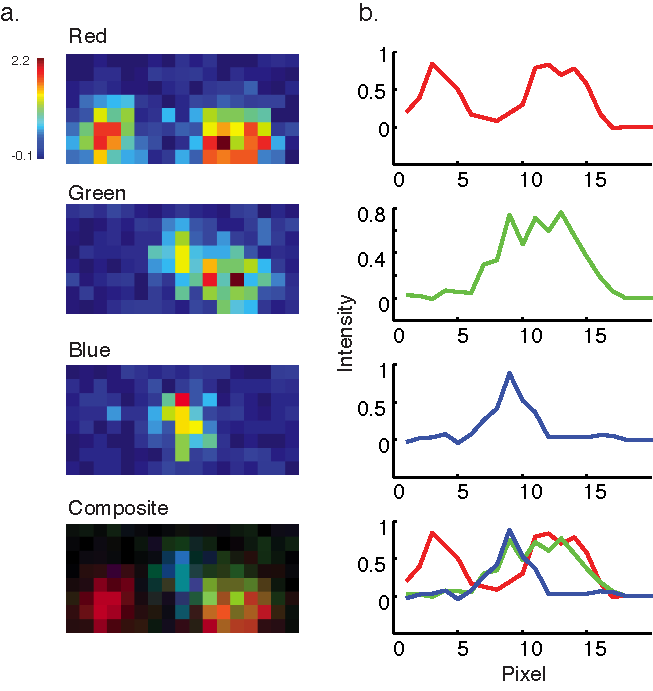
\includegraphics[width=\textwidth]{figures/fullpage}
% \caption[Short figure name.]{This is a full page figure using the FPfigure command. It takes up the whole page and the caption appears on the preceding page. Its useful for large figures. Harvard's rules about full page figures are tricky, but you don't have to worry about it because we took care of it for you. For example, the full figure is supposed to have a title in the same style as the caption but without the actual caption. The caption is supposed to appear alone on the preceding page with no other text. You do't have to worry about any of that. We have modified the fltpage package to make it work. This is a lengthy caption and it clearly would not fit on the same page as the figure. Note that you should only use the FPfigure command in instances where the figure really is too large. If the figure is small enough to fit by the caption than it does not produce the desired effect. Good luck with your thesis. I have to keep writing this to make the caption really long. LaTex is a lot of fun. You will enjoy working with it. Good luck on your post doctoral life! I am looking forward to mine. \label{fig:myFullPageFigure}}
% \end{FPfigure}
% \afterpage{\clearpage}

